\section{Техническое задание}
\subsection{Основание для разработки}

Полное наименование системы: "<Программная платформа для создания элементов графического\ пользовательского интерфейса">.
Основанием для разработки программы является приказ ректора ЮЗГУ от «04» апреля 2024 г. №1616-с «Об утверждении тем выпускных квалификационных работ».

\subsection{Назначение разработки}

Программно-информационная система предназначена для облегчения создания графических пользовательских интерфейсов в десктопных приложениях различного назначения.
В реализованном фреймворке должна быть обеспечена возможность создания новых элементов графического интерфейса сторонними разработчиками для своих приложений с различными функциональными возможностями.

\subsection{Требования к программной системе}

\subsubsection{Требования к данным программной системы}

На рисунке ~\ref{сoncept:image} представлена концептуальная модель данных программной системы в виде UML-диаграммы сущность-связь.

\begin{figure}[H]
	\includegraphics[width=1\linewidth]{сoncept}
	\caption{Концептуальная модель данных}
	\label{сoncept:image}
\end{figure}

Входными данными для фреймворка являются: изображения, файлы настроек, код программы, регистры и названия ресурсов.

Выходными данными являются: десктопное приложение.

\subsubsection{Функциональные требования к программной системе}

На основании анализа предметной области в программе должны быть реализованы следующие прецеденты:
\begin{enumerate}
	\item Добавление изображения.
	\item Добавление кнопки.
	\item Создание темы.
	\item Создание функции смены языка.
\end{enumerate}

\subsubsection{Моделирование вариантов использования}

Для разрабатываемого фреймворка была реализована модель, которая обеспечивает наглядное представление вариантов использования фреймворка.

Она помогает в физической разработке и детальном анализе взаимосвязей объектов. При построении диаграммы вариантов использования применяется унифицированный язык визуального моделирования UML\cite{uml}.(рисунок ~\ref{use:image}).

\begin{figure}[ht]
	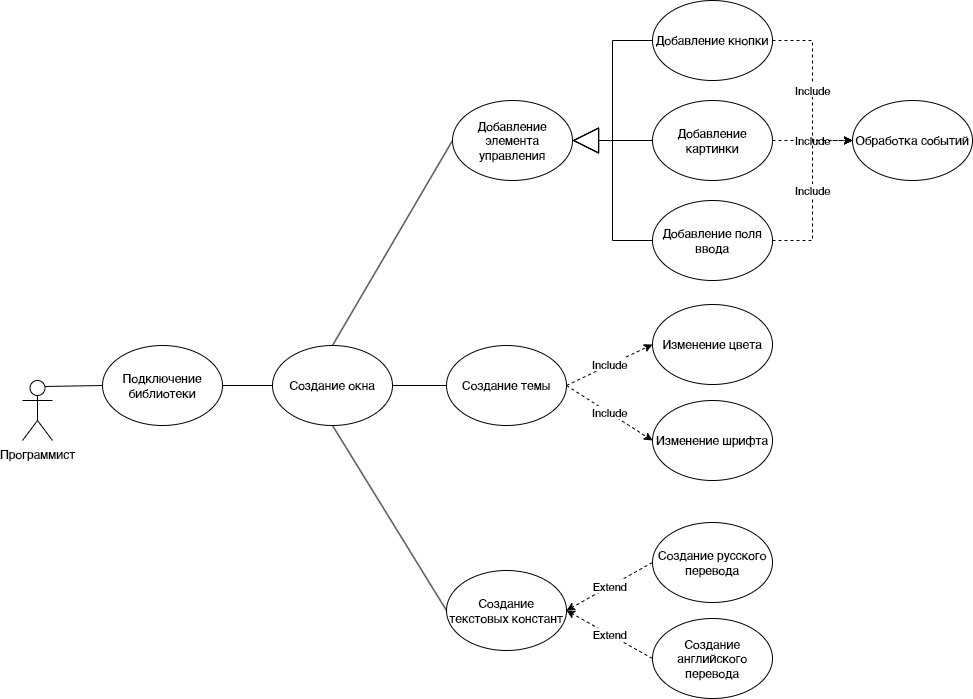
\includegraphics[width=1\linewidth]{use}
	\caption{Варианты использования фреймворка}
	\label{use:image}
\end{figure}

\subsubsection{Вариант использлвания "<Добавление изображения">}
Заинтересованные лица и их требования: пользователь желает добавить изображение.
Предусловие: пользователь создал папку images в папке res и создал нужные темы.
Постусловие: Изображение повилось в окне.

Основной успешный сценарий:
\begin{enumerate}
	\item Пользователь создал несколько вариантов изображений.
	\item Пользователь включил изображения в реестр.
	\item Пользователь добавил переменную изображения и приписал к ней реестр в файле заголовка.
	\item Пользователь прописал название ресурса и путь к изображению в файле ресурсов.
	\item Пользователь прописал изображение в файле темы.
	\item Пользователь добавил элемент управления с помощью метода add{\_}control() в коде.
	\item Пользователь прописал позицию в методе UpdateControlsPosition().
\end{enumerate}

\subsubsection{Вариант использлвания "<Добавление кнопки">}
Заинтересованные лица и их требования: пользователь желает добавить кнопку.
Предусловие: пользователь создал файл окна и файл темы.
Постусловие: создается ini файл в корневой папке проекта.

Основной успешный сценарий:
\begin{enumerate}
	\item Пользователь добавил переменную кнопки в файле заголовка.
	\item Пользователь прописал событие и связал его с помощью команды bind().
	\item Пользователь создал элемент управления с помощью метода add{\_}control() в коде.
	\item Пользователь прописал позицию в методе UpdateControlsPosition().
	\item Пользователь прописал кнопку в json-файле темы.
\end{enumerate}

\subsubsection{Вариант использлвания "<Создание темы">}
Заинтересованные лица и их требования: пользователь желает создать тему для своего проекта.
Предусловие: пользователь создал json-файл в папке res.
Постусловие: при нажатии кнопки сменяется тема.

Основной успешный сценарий:
\begin{enumerate}
	\item Пользователь создал несколько вариантов тем.
	\item Пользователь прописал название тем в реестре файла "<resources.h">.
	\item Пользователь прописал тип ресурса и путь к темам в файле формата "<.rc">.
	\item Пользователь добавил темы в методе set{\_}app{\_}themes() в файле "<main.cpp">.
	\item Пользователь выбрал первичную тему с помошью config.
	\item Пользователь создал элемент управления switch{\_}theme{\_}button.
\end{enumerate}

\subsubsection{Вариант использлвания "<Создание функции смены языка">}
Заинтересованные лица и их требования: пользователь желает создать файл для быстрой настройки окна и других переменных.
Предусловие: пользователь ввел команду создания файла конфигураций.
Постусловие: при нажатии на кнопку меняется язык.

Основной успешный сценарий:
\begin{enumerate}
	\item Пользователь создал несколько вариантов языка.
	\item Пользователь прописал название языка в реестре файла "<resources.h">.
	\item Пользователь прописал тип ресурса и путь к темам в файле формата "<.rc">.
	\item Пользователь добавил темы в методе set{\_}app{\_}locales() в файле "<main.cpp">.
	\item Пользователь выбрал первичную тему с помошью config.
	\item Пользователь создал элемент управления switch{\_}lang{\_}button.
	\item Пользователь связал язык с нужными элементами.
\end{enumerate}

\subsubsection{Требования к интерфейсу}
Фреймворк должен:
\begin{enumerate}
	\item Обеспечивать создание новых компонентов.
	\item Предоставлять общий интерфейс к подсистеме рисования.
	\item Предоставлять общий интерфейс к событиям. Любой компонент или пользователь может подписаться на любую группу сообщений, в том числе пользовательскую, с возможностью асинхронной отправки/получения сообщений.
	\item Принимать системные сообщения, реагировать на мышь, клавиатуру и прочие события.
	\item Открывать окна и отображать на них компоненты.
    \item Предоставлять систему текстовых констант для заголовков и надписей в зависимости от выбранного языка.
    \item Предоставлять систему тем для изменения шрифтов и цветовых акцентов в зависимости от выбранной темы.
\end{enumerate}

Модель простого окна представлена на рисунке ~\ref{window:image}.

\begin{figure}[ht]
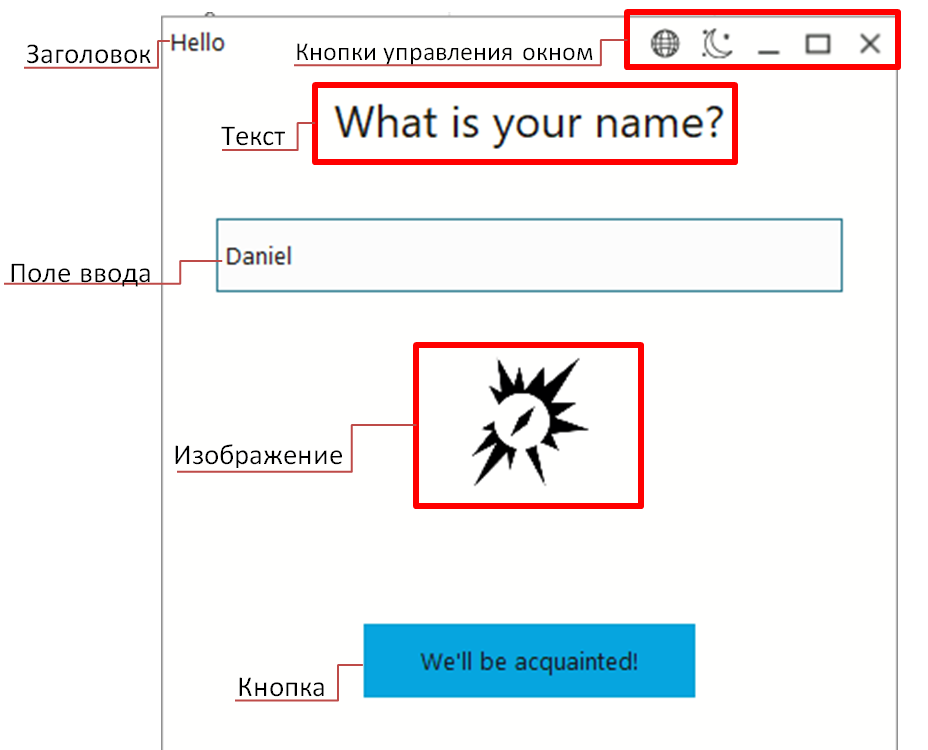
\includegraphics[width=1\linewidth]{window}
\caption{Общая схема простого окна}
\label{window:image}
\end{figure}
%\vspace{-\figureaboveskip} % двойной отступ не нужен (можно использовать, если раздел заканчивается картинкой)

В состав данного окна входят название программы, кнопки управления окном, такие как: кнопка смены темы, кнопка смены языка, кнопка свернуть окно, кнопка развернуть окно, кнопка закрыть окно, и другие элементы взаимодействия, такие как: поле для ввода текста, кнопка подтверждения ввода, различные изображения и текст.

\subsection{Нефункциональные требования к программной системе}

\subsubsection{Требования к надежности}
Приложение должно функционировать на всех разработанных тестах. Тесты требуется разработать на этапе рабочего проекта.
Приложение должено устойчиво функционировать при соблюдении гарантии устойчивого функционирования операционной системы. Под устойчивой работой ПК понимается непрерывное функционирование программы в отсутствии критических сбоев, приводящих к аварийному завершению.

\subsubsection{Требования к аппаратному обеспечению}

Для работы c фреймворком необходимо дисковое пространство не менее 38 Мб, свободная оперативная память в размере не менее 512 Мб, видеокарта с не менее 256 Мб видеопамяти, разрешение экрана не менее 1024*768, клавиатура, мышь.

\subsection{Требования к оформлению документации}

Требования к стадиям разработки программ и программной документации для вычислительных машин, комплексов и систем независимо от их назначения и области применения, этапам и содержанию работ устанавливаются ГОСТ 19.102–77.

Программная документация должна включать в себя:
\begin{enumerate}
	\item Анализ предметной области.
	\item Техническое задание.
	\item Технический проект.
	\item Рабочий проект.
\end{enumerate}
